%!TEX program = lualatex
\documentclass[a4paper,12pt,openany,oneside]{memoir}

\usepackage{microtype}
\usepackage[hmargin = 1.91cm, vmargin = 2.54cm]{geometry}
\usepackage{float}

\usepackage[no-math]{fontspec}
\setmainfont{STIXTwoText}[
    Path            = ./fonts/STIX2/   ,
    UprightFont     = *-Regular.otf    ,
    BoldFont        = *-Bold.otf       ,
    ItalicFont      = *-Italic.otf     ,
    BoldItalicFont  = *-BoldItalic.otf
    ]

\usepackage{unicode-math}
\setmathfont{STIXTwoMath.otf}[Path = ./fonts/STIX2/]

\setmonofont{FiraCode}[
    Path        = ./fonts/FiraCode/ ,
    UprightFont = *-Regular.ttf    ,
    BoldFont    = *-Bold.ttf     ,
    ]

\usepackage[usenames,svgnames]{xcolor}
\usepackage{icomma}
\usepackage{tocloft}
\usepackage{hyperref}
\usepackage{enumitem}
\usepackage{amsmath}
\usepackage{listings}
\usepackage[english,russian]{babel}


% Chapter header format
\renewcommand{\afterchapternum}{\hspace{1ex}}
\renewcommand{\chapnamefont}{\centering\bfseries\LARGE}
\renewcommand{\chapnumfont}{\centering\bfseries\LARGE}
\renewcommand{\chaptitlefont}{\centering\bfseries\LARGE}
\sethangfrom{\noindent #1}
\indentafterchapter

% Correct display of the new chapter and section formats with babel
\addto\captionsrussian{
    \renewcommand{\secheadstyle}{\centering\bfseries\Large\S\space}
    \renewcommand{\subsecheadstyle}{\centering\bfseries\large}
    \renewcommand{\contentsname}{\bfseries Содержание}
    \renewcommand{\chaptername}{\S}
    }
    
\pagestyle{plain}
\OnehalfSpacing

% Define new language style for C++
\lstdefinestyle{MyCPP}{
    language=C++ ,
    escapechar=\@ ,
    breaklines ,
    resetmargins=true ,
    keepspaces=true ,
    basicstyle=\ttfamily\small ,
    keywordstyle=\color{NavyBlue}\bfseries\ttfamily\small ,
    stringstyle=\color{Blue}\ttfamily\small ,
    commentstyle=\color{Green}\ttfamily\small ,
    morecomment=[l][\color{LimeGreen}]{\#} ,
    emph=[1]{cout,endl,std,string,ofstream,ifstream} ,
    emphstyle=[1]\color{ForestGreen}\bfseries\ttfamily\small ,
    literate=
        *{0}{{{\color{Magenta}0}}}1
        {1}{{{\color{Magenta}1}}}1
        {2}{{{\color{Magenta}2}}}1
        {3}{{{\color{Magenta}3}}}1
        {4}{{{\color{Magenta}4}}}1
        {5}{{{\color{Magenta}5}}}1
        {6}{{{\color{Magenta}6}}}1
        {7}{{{\color{Magenta}7}}}1
        {8}{{{\color{Magenta}8}}}1
        {9}{{{\color{Magenta}9}}}1
        {(}{{{\color{Red}(}}}1
        %fix right parenthesis ) not being colored
        {')}{{{\color{Red})}}}1
        %
        {[}{{{\color{Red}[}}}1
        {]}{{{\color{Red}]}}}1
        {=}{{{\color{Red}=}}}1
        {;}{{{\color{Red};}}}1
        {<}{{{\color{Red}<}}}1
        {.}{{{\color{Red}.}}}1
        {>}{{{\color{Red}>}}}1
        {+}{{{\color{Red}+}}}1
        {-}{{{\color{Red}-}}}1
        {*}{{{\color{Red}*}}}1
        {\&}{{{\color{Red}\&}}}1
        {\%}{{{\color{Red}\%}}}1
}

\begin{document}
% New section numbering format
\setsecnumformat{\csname the#1\endcsname \space}
% Quick command for using mono bold font
\newcommand{\monobf}[1]{{\ttfamily\textbf{#1}}}
% Set language style for C++
\lstset{style=MyCPP}

\tableofcontents*
\addcontentsline{toc}{chapter}{Предисловие}

\chapter{Установка редактора исходного кода Code::Blocks}
Для написания собственных программ на языке программирования C\texttt{++} необходимо установить любую из возможных сред разработки. Например, свободную кроссплатформенную среду разработки --- \textbf{Code::Blocks}.
\begin{itemize}
    \item Скачиваем дистрибутив с сайта {\color{Blue}\href{https://www.codeblocks.org/downloads/binaries/#imagesoswindows48pnglogo-microsoft-windows}{codeblocks.org}}.
    \item После установки на рабочем столе появляется иконка с одноименным названием, или же в меню \textbf{Пуск$\rightarrow$Все программы}.
    \item В открывшемся окне выбираем \textbf{Create a new project}
    \begin{figure}[H]
        \centering
        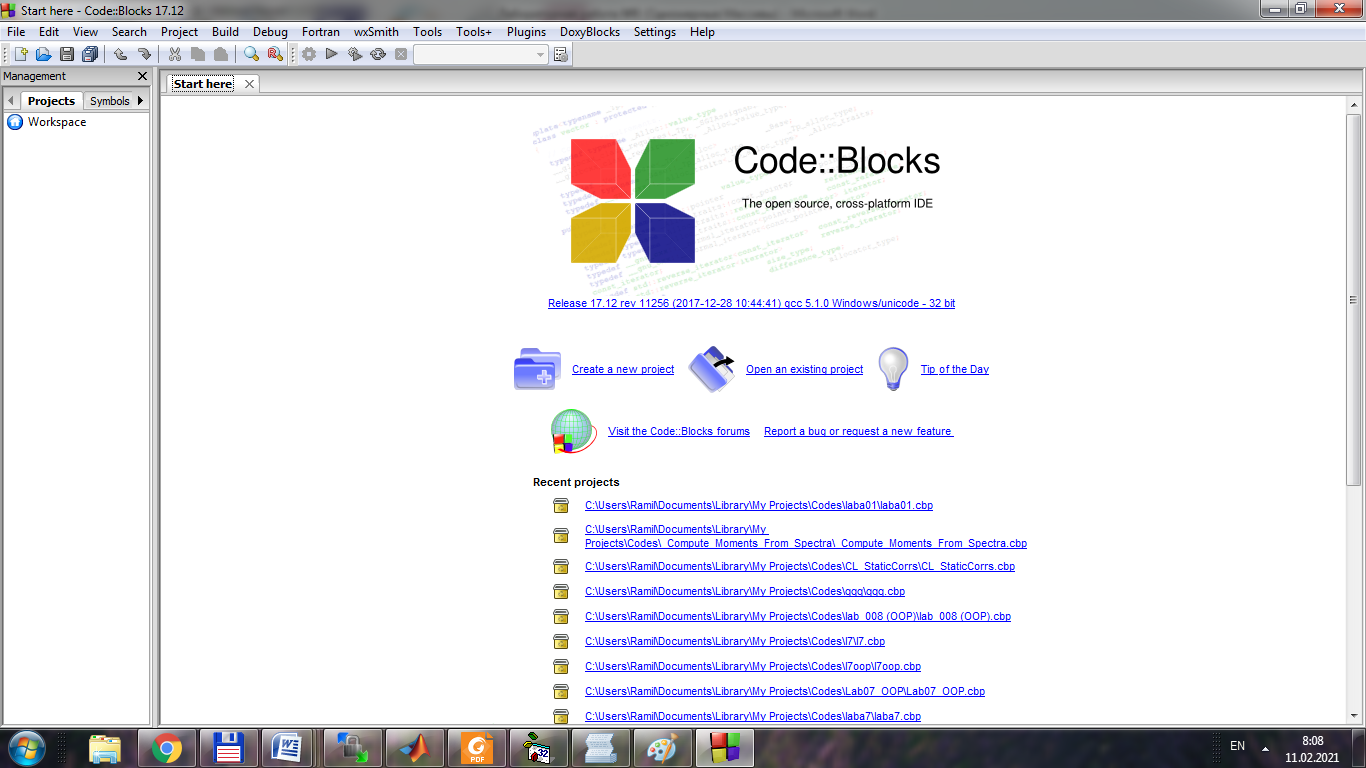
\includegraphics[width=.9\linewidth]{figures/CodeBlocks-1.png}
        \caption{Запуск программы Code::Blocks}
        \label{CodeBlocks-1}
    \end{figure}
    \item Выбираем иконку \textbf{Console Application}
    \begin{figure}[H]
        \centering
        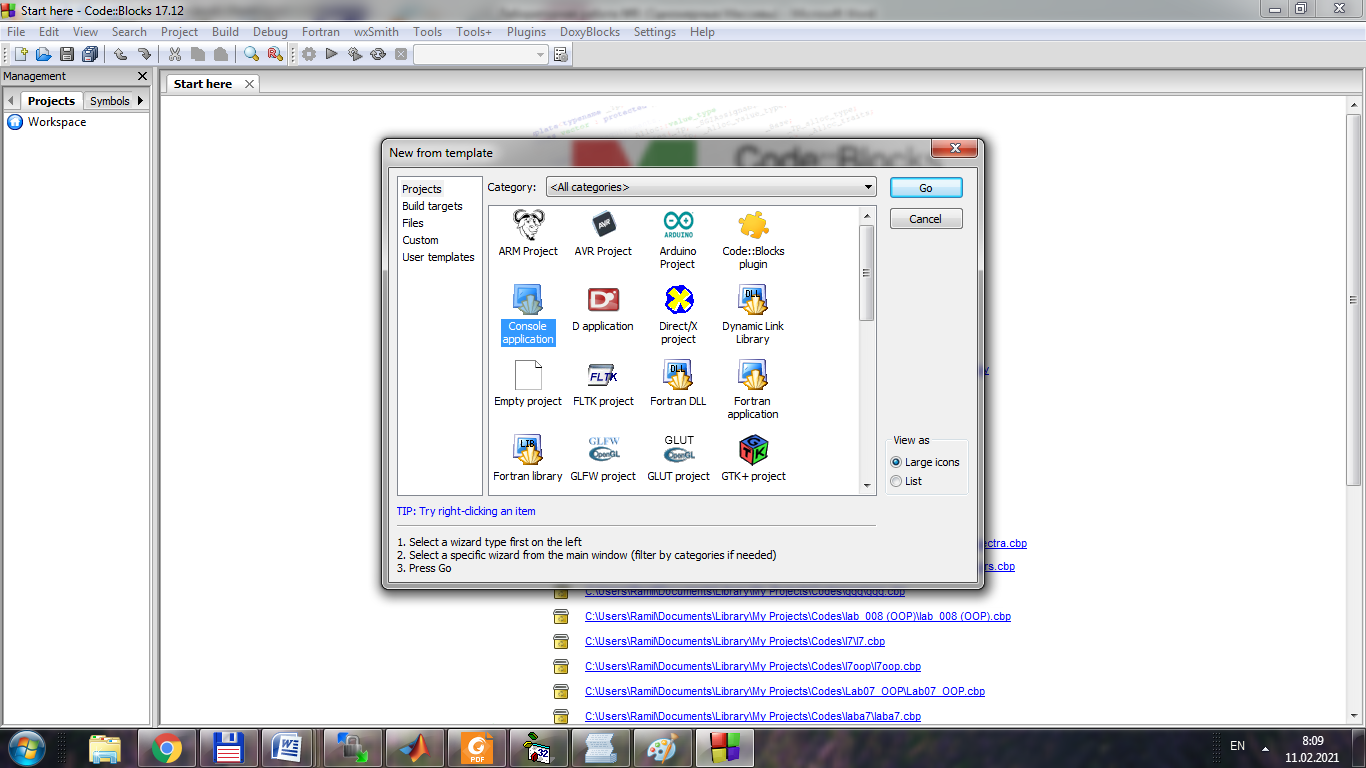
\includegraphics[width=.9\linewidth]{figures/CodeBlocks-2.png}
        \caption{Окно выбора иконки Console Application}
        \label{CodeBlocks-2}
    \end{figure}
    \item Выбираем \textbf{C\texttt{++}}
    \begin{figure}[H]
        \centering
        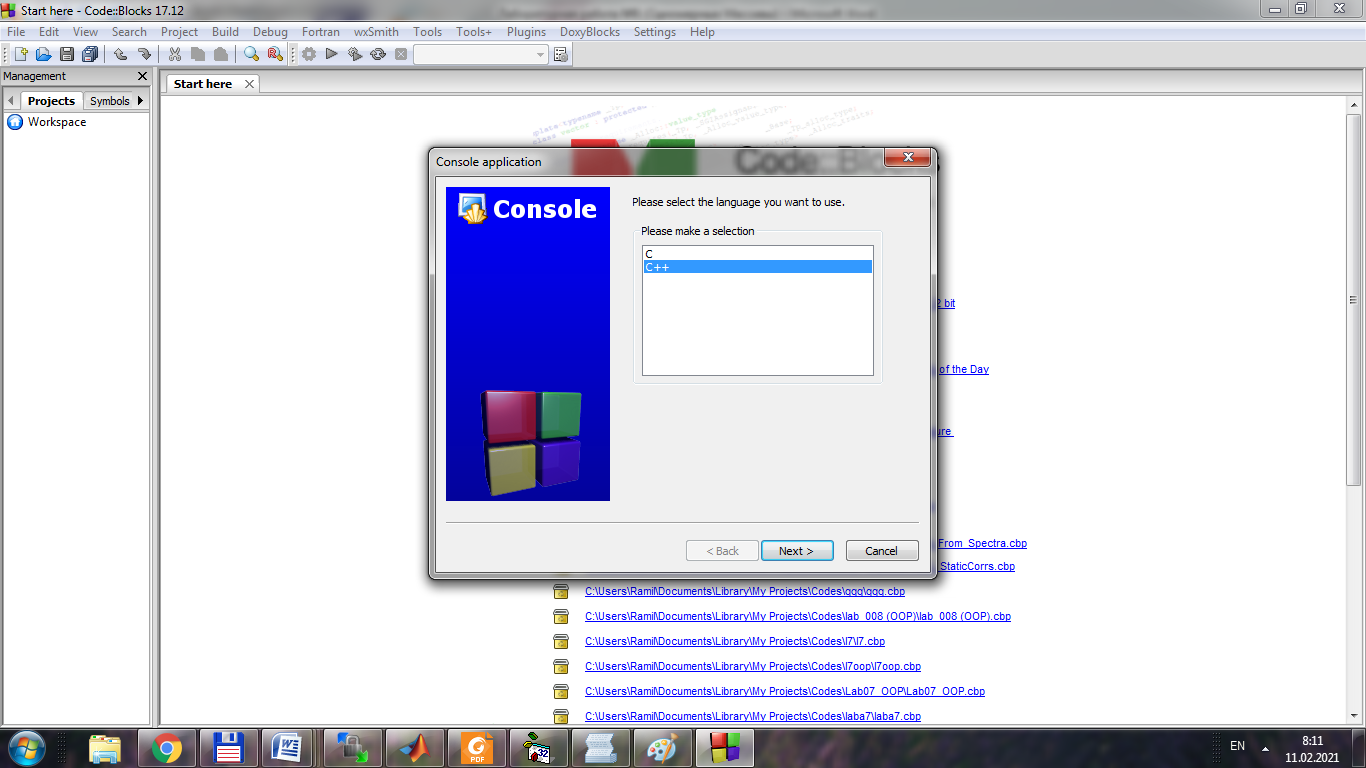
\includegraphics[width=.9\linewidth]{figures/CodeBlocks-3.png}
        \caption{Выбор языка C\texttt{++}}
        \label{CodeBlocks-3}
    \end{figure}
    \item Пишем имя проекта, например, \textbf{\_\_lab01}
    \begin{figure}[H]
        \centering
        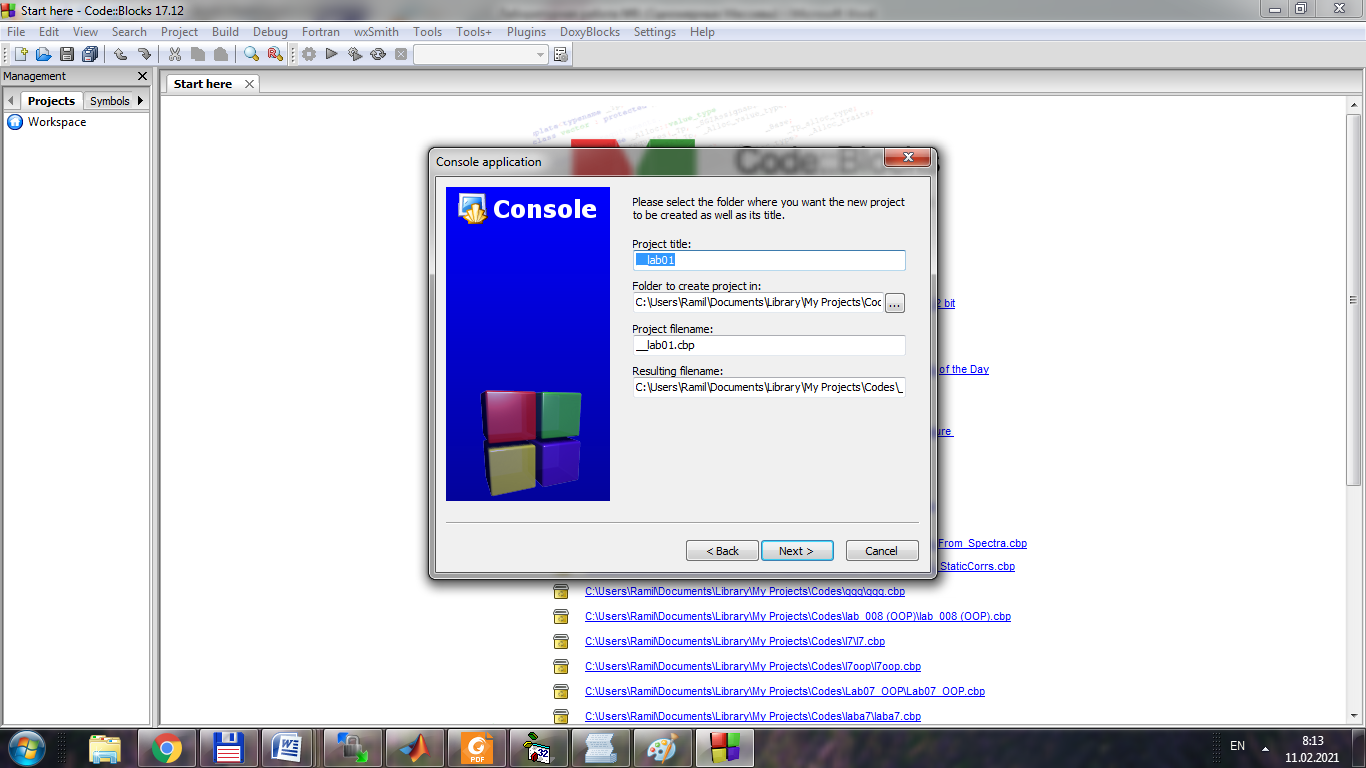
\includegraphics[width=.9\linewidth]{figures/CodeBlocks-4.png}
        \caption{Ввод имени проекта}
        \label{CodeBlocks-4}
    \end{figure}
    \item Далее, соглашаемся на все предложенные варианты, и кликаем на вкладку \textbf{Sources}$\rightarrow$ \textbf{main.cpp}. В результате, получаем следующее окно и шаблон программы \textbf{Hello, world!}
    \begin{figure}[H]
        \centering
        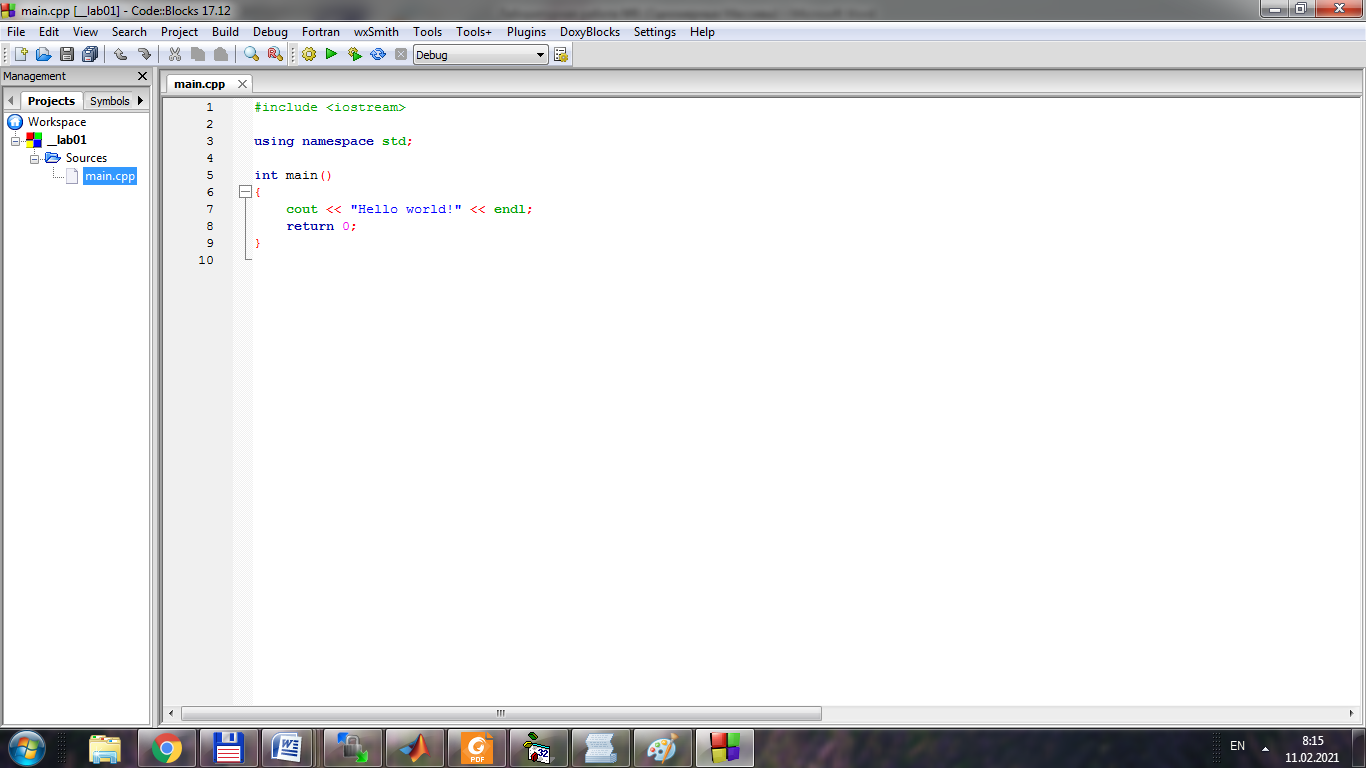
\includegraphics[width=.9\linewidth]{figures/CodeBlocks-5.png}
        \caption{Программа <<Hello, world!>> в окне редактора исходного кода}
        \label{CodeBlocks-5}
    \end{figure}
    \item Для компиляции и запуска программы нажимаем на клавишу \textbf{F9} (\textbf{Build and run}).
\end{itemize}
\chapter{Массивы}

\section{Одномерные массивы}
\begin{enumerate}[leftmargin=*]
    \item Дан массив вещественных чисел. Найдите сумму отрицательных элементов массива.
    \item Найдите произведение элементов массива с нечетными номерами.
    \item Дан массив целых чисел. Количество запросить с клавиатуры. Найти максимальный (минимальный) элемент массива и его номер, при условии, что все элементы различные.
    \item Найдите наименьший четный элемент массива. Если такого нет, то выведите первый элемент.
    \item Преобразовать массив так, чтобы сначала шли нулевые элементы, а затем все остальные.
    \item Ввести массив, в котором только два одинаковых элемента. Определить их местоположение.
    \item Ввести два массива действительных чисел. Определить максимальные элементы в каждом массиве и поменять их местами.
    \item Задан целочисленный массив. Определить процентное содержание элементов, превышающих среднеарифметическое всех элементов массива.
    \item Выполнить сортировку массива по возрастанию (убыванию).
    \item Дан массив из 10 элементов. Первые 4 упорядочить по возрастанию, последние 4 по убыванию.
\end{enumerate}
\section{Сортировка и упорядочение массивов}
\begin{enumerate}[leftmargin=*]
    \item Создайте матрицу случайных чисел размерности $n \times m$ в диапазоне $[1;10]$.
    \item Дана квадратная матрица. Вывести на экран элементы, стоящие на диагонали.
    \item Дана матрица. Вывести на экран все нечетные столбцы, у которых первый элемент меньше последнего.
    \item Дана матрица $N\times M$ случайных чисел. Отсортировать элементы главной диагонали матрицы по убыванию.
    \item Дана матрица $N\times M$ случайных чисел. Упорядочить первый столбец матрицы по возрастанию, а последний столбец --- по убыванию.
    \item Дан массив из 10 элементов. Отсортируйте отдельно элементы от 0-го по 2-й, с 3-го по 5-й и с 6-го по 9.
    \item Дан трехмерный массив $N\times M\times K$ случайных чисел $(N, M, K>5)$. Отсортируйте матрицу $N\times M$ при $K=2$ и выведите её на экран монитора.
    \item Дан массив 20 целых чисел на отрезке $[-2;5]$. Упорядочить массив, удалив нули со сдвигом влево, ненулевыми элементами.
    \item Дан массив 20 целых чисел на отрезке $[-5;5]$. Упорядочить массив, удалив повторяющиеся элементы.
    \item Дан массив. Найдите два соседних элемента, сумма которых минимальна.
    \item В данном массиве найдите количество чисел, соседи у которых отличаются более чем в 2 раза.
    \item Дана матрица. Вывести на экран все четные строки.
    \item Найдите сумму номеров минимального и максимального элементов массива.
    \item Введите одномерный целочисленный массив. Найдите наибольший нечетный элемент. Далее осуществите циклический сдвиг влево элементов, стоящих справа от найденного максимума.
    \item Дан массив размером nxn, элементы которого целые числа. Для каждого столбца подсчитать сумму отрицательных элементов и записать данные в текстовый файл.
    \item В двумерном массиве, элементы которого целые числа, удалить все столбцы, в которых первый элемент больше последнего. Результат записать в файл.
\end{enumerate}
\chapter{Файлы}
\section{Лабораторная работа 1}
\begin{enumerate}[leftmargin=*]
    \item Создайте матрицу \monobf{x[n][n]} случайных чисел. Сохраните все элементы матрицы в файл с названием \monobf{Matrix.txt}. Считайте содержимое файла \monobf{Matrix.txt} в новый массив \monobf{y[n][n]} и выведите его на экран дисплея.
    \item Напишите программу, которая считывала бы элементы главной диагонали матрицы из файла \monobf{Matrix.txt}.
    \item Напишите программу, которая удаляла бы $k$-столбец ($1<k<M$) в файле \monobf{Matrix.txt}.
    \item Напишите программу, которая считывала бы элементы матрицы из файла \monobf{Matrix.txt} и записывала бы их в массив, соответствующего размера. Отсортируйте все столбцы матрицы по убыванию. Полученный массив запишите в файл \monobf{Matrix\_Sort.txt}.
    \item Дан текстовый файл, содержащий целые числа. Удалить из него все четные числа. 
    \item В данном текстовом файле удалить все слова, которые содержат хотя бы одну цифру. 
    \item Напишите программу, которая считывала бы саму себя и выводила бы на экран дисплея исходный текст программы в обратном порядке.
    \item Имеется файл с текстом. Осуществить шифрование данного текста в новый файл. Осуществить расшифровку полученного текста.
\end{enumerate}

\end{document}